\subsection{要求獲得}

\term{要求獲得}とは、候補となる要求を表面化させる活動である。英語では \,\en{Requirements Elicitation}\, と呼ばれる。直訳すれば「引き出し」であり、相手が最初から明確に言語化できるとは限らないニーズを、質問、観察、試作、資料調査などで明らかにする活動である。

要求獲得が不十分だと、不完全な要求が残る。完全性を保証することは難しいが、適切な源泉を見つけ、複数の技法を組み合わせることで、不完全性を減らせる。

\subsubsection{要求の源泉}

要求は多くの源泉から来る。人に由来する源泉と、人以外に由来する源泉の両方を考える必要がある。

\par\smallskip\noindent\refstepcounter{table}\label{tab:ch01-06}\textbf{表 \thetable: 第01章 ソフトウェア要求 表06}\par\smallskip
\begin{tabularx}{0.97\linewidth}{@{}p{.27\linewidth}X@{}}
\toprule
源泉 & 例 \\
\midrule
\term{顧客} & ソフトウェア開発に費用を出す人・組織。 \\
\term{利用者} & ソフトウェアを直接または間接に使う人。利用頻度、権限、熟練度で分類できる。 \\
\term{業務専門家} & 対象業務、規制、現場作業に詳しい人。 \\
\term{運用担当} & 本番環境、監視、障害対応、バックアップなどに責任を持つ人。 \\
\term{サポート担当} & 利用者からの問い合わせや障害報告を受ける人。 \\
\term{規制当局・専門団体} & 法令、標準、ガイドラインを通じて要求を課す組織。 \\
\term{開発者} & 技術的制約、保守性、開発効率に関する要求を示すことがある。 \\
\bottomrule
\end{tabularx}

また、要求は人からだけではなく、文書、既存システム、業務方針、計算環境、競合製品、障害履歴、標準、法規制からも得られる。

\MiniBox{利害関係者分析}{利害関係者分析とは、関係する人や組織をできるだけ漏れなく見つけ、代表性の偏りを減らす活動である。声の大きい利用者だけから要求を集めると、少数派や運用担当の重要な要求を見落としやすい。}

\subsubsection{要求獲得技法}

要求獲得には多くの技法がある。技法は相手や目的によって使い分ける。

\par\smallskip\noindent\refstepcounter{table}\label{tab:ch01-07}\textbf{表 \thetable: 第01章 ソフトウェア要求 表07}\par\smallskip
\begin{tabularx}{0.97\linewidth}{@{}p{.25\linewidth}X@{}}
\toprule
技法 & 何に向いているか \\
\midrule
\term{面接} & 個別の経験、例外処理、暗黙知を聞き出す。 \\
\term{会議・討議} & 複数の関係者で認識を合わせる。 \\
\term{促進付きワークショップ} & 利害関係者を集め、短時間で合意形成や要求整理を行う。 \\
\term{質問票・市場調査} & 多数の人から傾向を集める。 \\
\term{観察} & 現場作業や実際の利用状況を確認する。 \\
\term{徒弟型学習} & ソフトウェア技術者が実際の作業を体験し、暗黙知を得る。 \\
\term{試作} & 画面や操作感を具体化し、利用者から反応を得る。 \\
\term{ユーザーストーリーマッピング} & 利用者の行動の流れに沿って機能を整理する。 \\
\term{文献・標準調査} & 法規制、標準、既存仕様に基づく要求を見つける。 \\
\bottomrule
\end{tabularx}

\begin{figure}[htbp]
\centering
\IfFileExists{assets/generated_figures/ch01/fig-ch01-06.png}{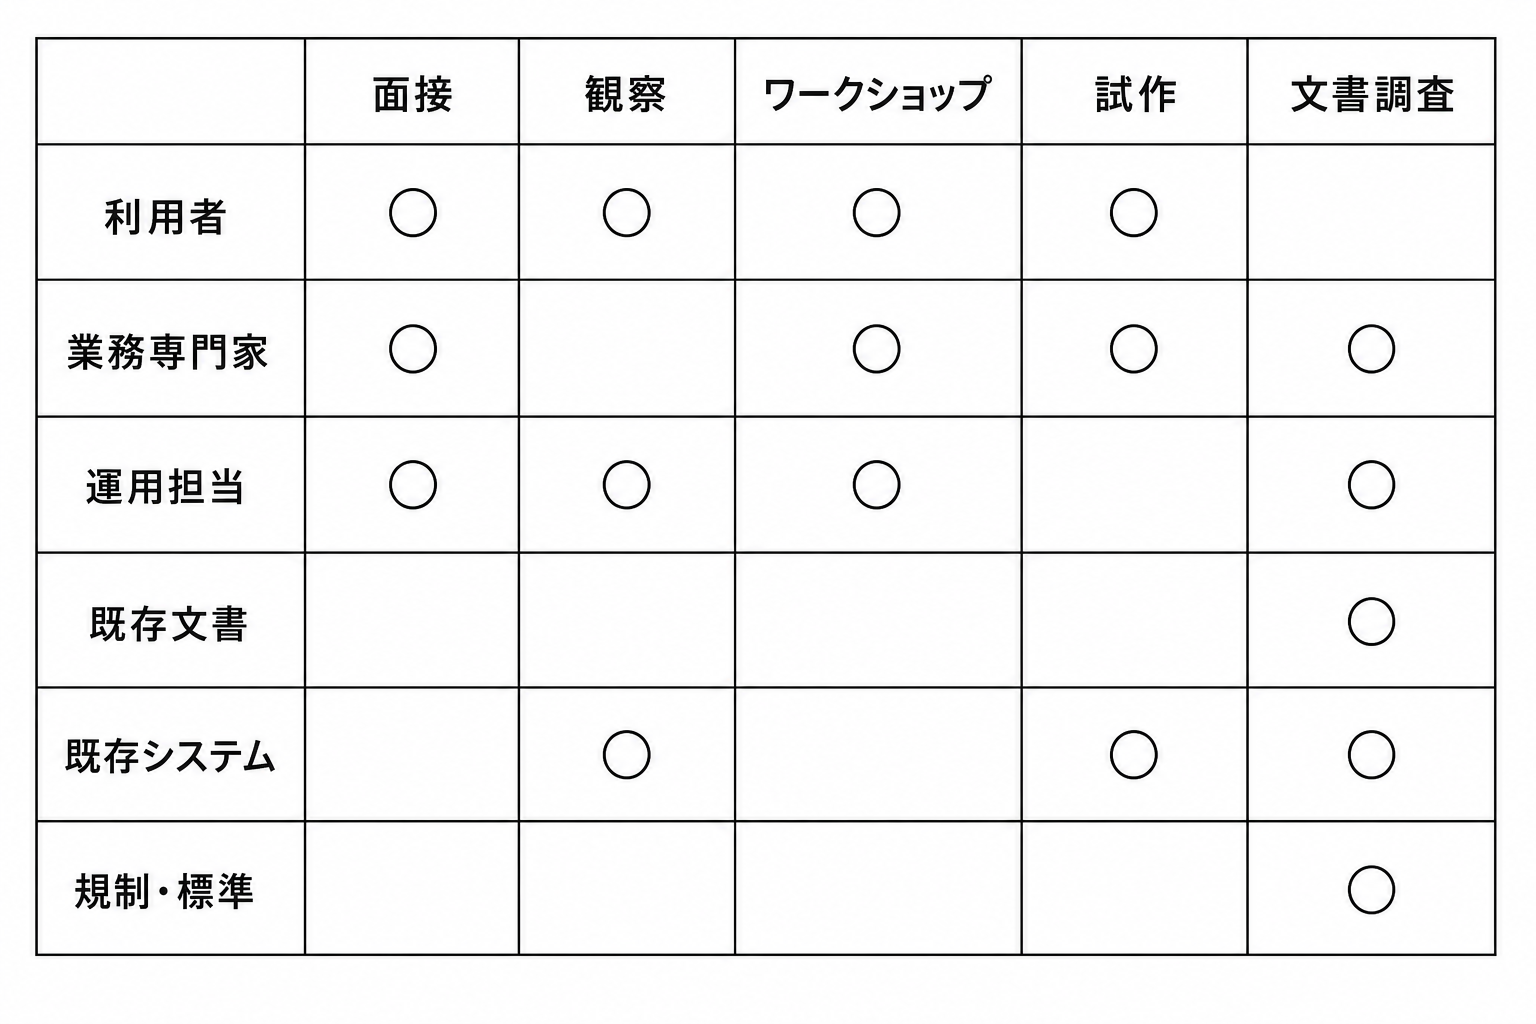
\includegraphics[width=0.96\linewidth]{assets/generated_figures/ch01/fig-ch01-06.png}}{\fbox{\parbox[c][48mm][c]{0.9\linewidth}{\centering 画像生成待ち\\要求の源泉と獲得技法の対応図}}}
\caption{要求の源泉と獲得技法の対応図}
\label{fig:ch01-06}
\end{figure}

要求獲得は受け身の活動ではない。利用者は自分の作業をうまく説明できないことがある。重要な情報を当然のこととして言わないこともある。したがって、技術者は「言われたことを書くだけ」ではなく、質問し、観察し、仮説を作り、確認する必要がある。
